\documentclass[12pt]{article}
\usepackage[czech]{babel}
\usepackage[utf8]{inputenc}
\usepackage[plainpages=false,pdfpagelabels,unicode]{hyperref}
\usepackage[pdftex]{graphicx}
\usepackage[margin=2cm, includefoot]{geometry}

\begin{document}

\title{Praktikum z fyziky plazmatu \\
Paschenův zákon}
\author{Pavel Ondračka}
\maketitle

\section{Úvod}
Svazek elektronů, vznikajících fotoemisí z katody vlivem ultrafialového záření urychlujeme homogenním elektrickým polem. Elektrony při průchodu plynem způsobují ionizaci a jejich počet exponenciálně vzrůstá. Pro hustotu elektronů platí $n_\mathrm{e}=n_0 \mathrm{e}^{\alpha d}$.
Koeficient $\alpha$ závisí na intenzitě elektrického pole a na tlaku (na $E$ závisí energie získaná na střední volné dráze, na tlaku pak samotná velikost střední volné dráhy). Při vzniku elektronové laviny také vzniká $n_0 (\mathrm{e}^{\alpha d} - 1)$ iontů. Podmínka pro zapálení výboje je $\gamma (\mathrm{e}^{\alpha d} - 1)=1$, kde $\gamma$ je koeficient sekundární emise. 
Townsendův ionizační koeficient závisí na tlaku a intenzitě el. pole vztahem: $\frac{\alpha}{p} = A \mathrm{e}^{\frac{-B p}{E}}$,
kde $A$ a $B$ jsou konstanty. Kombinací výše uvedených vzorců lze odvodit Paschenův zákon pro zápalné napětí.
\begin{equation}
U_\mathrm{z} = B \frac{pd}{C' + \ln{pd}}
\end{equation}
Schéma pro měření Paschenova zákona je na obrázku \ref{schema1}.

\begin{figure}[htbp]
\begin{center}

\includegraphics[width=6cm]{nakres1.pdf}
\caption{Schéma aparatury pro měření zápalného napětí}
\end{center}
\label{schema1}
\end{figure}

Elektrická vodivost plynu není konstantní ale mění se v závislosti na proudu procházejícím výbojem.
Na obrázku \ref{VA} je znázorněna VA charakteristika samostatného výboje. V některých oblastech charakteristiky proud vzrůstá při konstantním napětí na elektrodách a dokonce i při klesajícím napětí. Tento jev můžeme vysvětlit vznikem prostorového náboje a změnou původního elektrického pole vytvářeného napětím na elektrodách. Je-li tvar pole vzniklého v důsledku prostorového náboje takový, že ionizace ve výboji vzrůstá, pak proud samovolně narůstá. Přitom může napětí na elektrodách klesat, dostáváme pak klesající část VA charakteristiky (oblast BC). V opačném případě, když elektrické pole vytvořené prostorovým nábojem vytváří horší podmínky ionizace, pak chceme-li zvýšit proud výbojem, je nutné zvýšit napětí na elektrodách (oblast AB). Zvyšování proudu v oblasti CD nelze vysvětlit vzrůstem driftové rychlosti nabitých částic, neboť se zde nemění napětí na elektrodách. Musí se tedy měnit celkový počet částic procházející průřezem trubice.

\begin{figure}[htbp]
\begin{center}

\includegraphics[width=8cm]{VA.pdf}
\caption{VA charakteristika samostatného výboje}
\label{VA}
\end{center}
\end{figure}

Napětí na výbojce se skládá z napětí na katodové oblasti a ze spádu napětí na kladném sloupci. Při malých proudech zůstává katodový spád potenciálu konstantní, napětí na kladném sloupci však klesá s rostoucím proudem. Protože v kladném sloupci klesá intenzita pole, musí zde být vzrůst proudu způsoben velmi rychlým růstem koncentrace nabitých částic. Vzroste-li proud natolik, že celá katoda je pokryta záporným světlem, přecházíme do oblasti anomálního doutnavého výboje. Napětí na katodové oblasti vzrůstá. Tento vzrůst napětí je větší než pokles na kladném sloupci. Důsledkem je vzrůstající část VA charakteristiky v oblasti DE. Oblast EF odpovídá přechodu v obloukový výboj. Schéma aparatury pro měření VA charakteristiky je na obrázku \ref{schema2}.

\begin{figure}[htbp]
\begin{center}

\includegraphics[width=6cm]{nakres3.pdf}
\caption{Schéma aparatury pro měření VA charakteristiky}
\label{schema2}
\end{center}
\end{figure}

Pod pojmem katodový spád potenciálu rozumíme napětí mezi hranicí záporného světla a katodou. Stanovení katodového spádu provedeme tak, že za konstantní proudu budeme přibližovat anodu ke katodě a odečítat napětí v závislosti na vzdálenosti elektrod. Jakmile se dostane anoda do oblasti záporného světla, zmizí anodové světlo. Při další zmenšování vzdálenosti elektrod začne dosud klesající napětí vzrůstat. Vzrůst napětí lze vysvětlit ztížením ionizace v důsledku toho, že zmizí záření, které hraje důležitou roli v mechanismu vytváření katodového spádu. Schéma aparatury pro měření katodového spádu je na obrázku \ref{schema3}.


\begin{figure}[htbp]
\begin{center}

\includegraphics[width=6cm]{nakres2.pdf}
\caption{Schéma aparatury pro měření katodového spádu}
\label{schema3}
\end{center}
\end{figure}



\section{Měření}
\subsection{Ověřte Paschenův zákon na výbojce s pohyblivými elektrodami. Znázorněte závislost zápalného napětí jako funkce součinu tlaku a vzdálenosti elektrod.}
Měření bylo prováděno prvně pro konstantní tlak 150\,Pa a různé vzdálenosti elektrod, následně pro vzdálenost elektrod 0,8\,cm a různé tlaky. Výsledky měření jsou na obrázku \ref{graph1} a v tabulce \ref{paschentable}. Fitováním naměřených dat byly získány hodnoty $B$ a $C'$
\begin{center}
$B = 464\pm 52\,\mathrm{V\,Pa^{-1}\,m^{-1}}$\\
$C' = 1,36 \pm 0,05 $
\end{center}

\begin{table}[htbp]
\begin{center}
\begin{tabular}{ccccccc}
\multicolumn{3}{c}{\textbf{konstantní p = 150\,Pa}} &  & \multicolumn{3}{c}{\textbf{konstantní \emph{d} = 0,8\,cm}} \\
$d$[cm] & $p d$ [m.Pa]& $U_\mathrm{v}$[V] &  & $p$[Pa] & $p d$ [m.Pa] & $U_\mathrm{v}$[V] \\
5,2 & 7,8 & 930 &  & 40 & 0,32 & 900 \\
4,2 & 6,3 & 900 &  & 50 & 0,4 & 700 \\
3,2 & 4,8 & 780 &  & 100 & 0,8 & 400 \\
2,7 & 4,05 & 700 &  & 200 & 1,6 & 500 \\
2,2 & 3,3 & 600 &  & 300 & 2,4 & 550 \\
1,7 & 2,55 & 550 &  & 400 & 3,2 & 600 \\
1,2 & 1,8 & 500 &  & 500 & 4 & 650 \\
1 & 1,5 & 500 &  & 700 & 5,6 & 750 \\
0,8 & 1,2 & 450 &  \multicolumn{4}{l}{} \\
0,6 & 0,9 & 400 &  \multicolumn{4}{l}{} \\
0,4 & 0,6 & 400 &   \multicolumn{4}{l}{} \\
0,3 & 0,45 & 450 &  \multicolumn{4}{l}{} \\
0,2 & 0,3 & 600 &  \multicolumn{4}{l}{} \\
0,1 & 0,15 & 900 &   \multicolumn{4}{l}{} \\
\end{tabular}
\caption{Ověřování Paschenova zákona}
\label{paschentable}
\end{center}
\end{table}

\begin{figure}[htbp]
\begin{center}
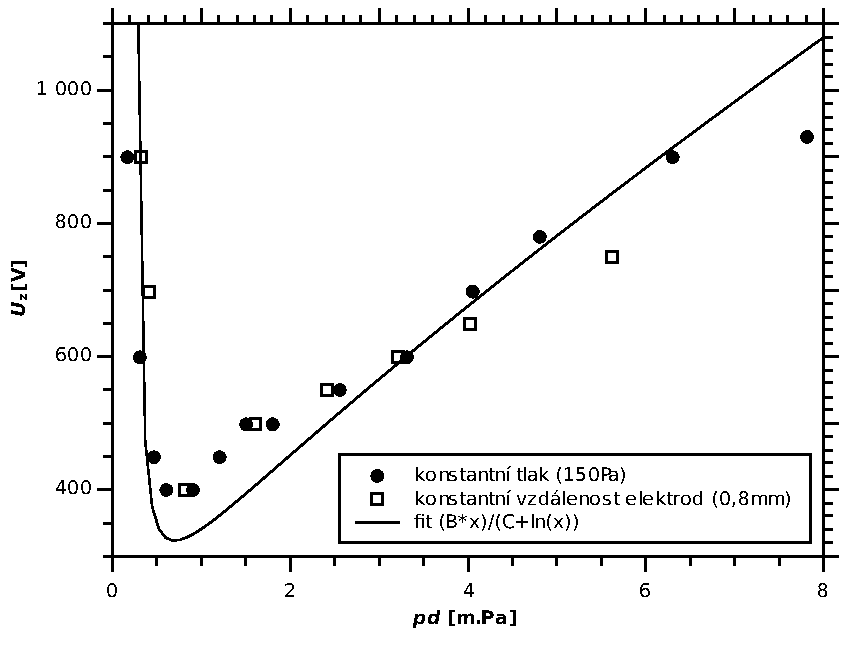
\includegraphics[width=12cm]{Graph1.pdf}
\caption{Závislost zápalného napětí na součinu tlaku a vzdálenosti elektrod}
\label{graph1}
\end{center}
\end{figure}


\subsection{Naměřte normální katodový spád potenciálu v doutnavém výboji}
Naměřený katodový spád je na obrázku \ref{graph2}. Katodový spád potenciálu určíme přímým odečtením z grafu. Pro $I_\mathrm{v} = $1,9\,mA a $p = $200\,Pa je $U_\mathrm{k} =$ 379\,V, pro $I_\mathrm{v} = $1,8\,mA a $p = $100\,Pa je $U_\mathrm{k} =$ 426\,V.

\begin{figure}[htbp]
\begin{center}
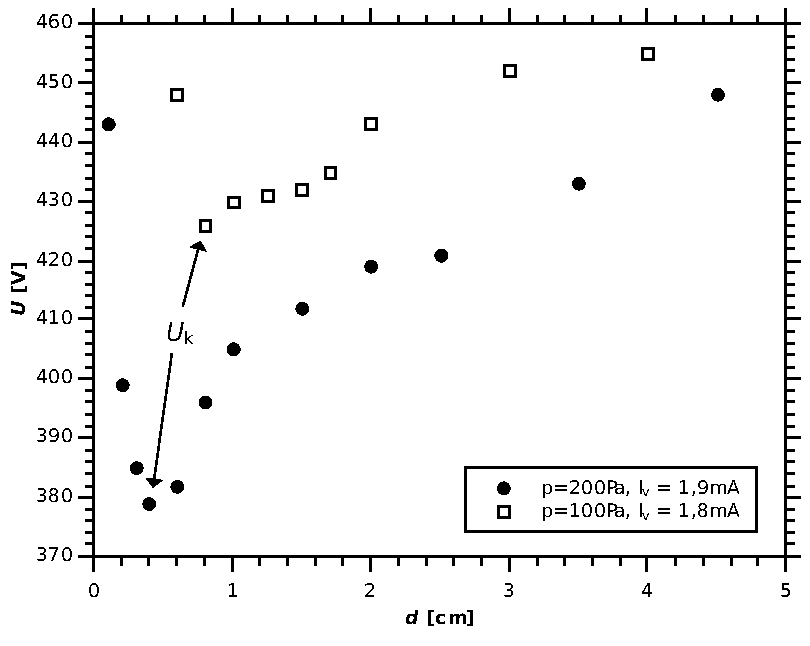
\includegraphics[width=12cm]{Graph2.pdf}
\caption{Katodový spád potenciálu v doutnavém výboji}
\label{graph2}
\end{center}
\end{figure}

\subsection{Naměřte VA charakteristiku samostatného výboje}
VA charakteristika byla měřena nepřímo. Bylo měřeno napětí na zdroji, napětí mezi elektrodami bylo vypočítáno jako $U_\mathrm{v} = U_\mathrm{zdroj} - I_\mathrm{v}R$, $U_\mathrm{zdroj}$ bylo po celou dobu měření 930\,V, VA charakteristika je na obrázku \ref{graph3} a v tabulce \ref{VA2}.

\begin{figure}[htbp]
\begin{center}
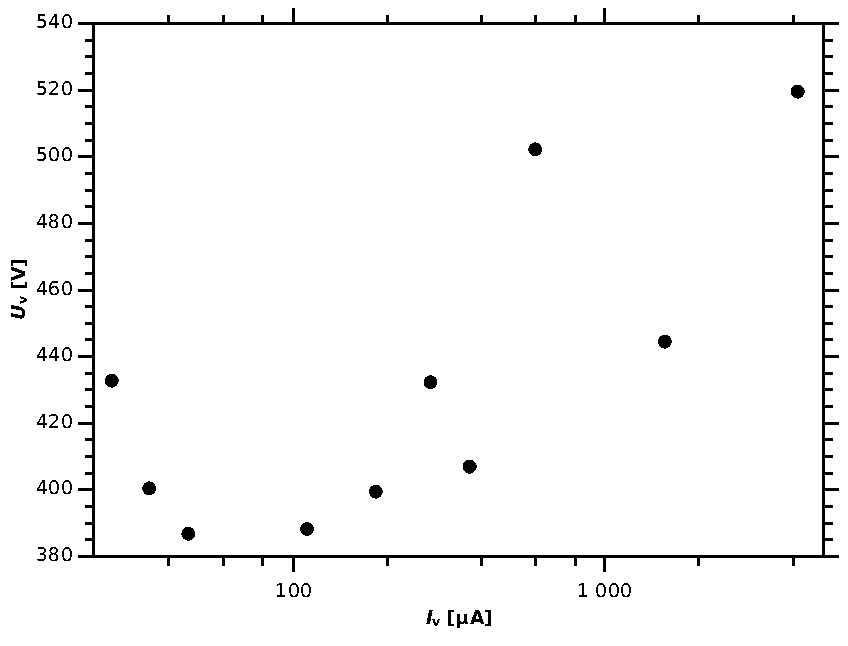
\includegraphics[width=12cm]{Graph3.pdf}
\caption{Naměřená VA charakteristika}
\label{graph3}
\end{center}
\end{figure}

\begin{table}[htbp]
\begin{center}
\begin{tabular}{ccc}
\hline
{$R [\mathrm{M\Omega]}$} & {$I_\mathrm{v} [\mathrm{\mu A]}$} & {$U_\mathrm{v} \mathrm{[V]}$} \\
\hline \hline
0,1 & 4100 & 520 \\
0,315 & 1540 & 444,9 \\
0,72 & 594 & 502,3 \\
1,428 & 366 & 407,3 \\
1,809 & 275 & 432,5 \\
2,88 & 184,1 & 399,7 \\
4,89 & 110,7 & 388,6 \\
11,8 & 46 & 387,2 \\
15,3 & 34,6 & 400,6 \\
19,04 & 26,1 & 433,0 \\
22,44 & 0 & 930 \\
\hline
\end{tabular}
\caption{VA charakteristika}
\label{VA2}
\end{center}
\end{table}



\section{Závěr}
Měření proběhlo úspěšně. Průběh závislosti zápalného napětí na součinu vzdáleností elektrod a tlaku velmi dobře odpovídá teoretickým očekáváním. Data dobře souhlasí s fitem, mírná odchylka je pouze v oblasti minima, to je dle mého názoru hlavně způsobeno nejhorší přesností voltmetru právě pro nízká napětí, kdy je chyba při odečítání ze stupnice voltmetru odhadem $\pm$50-100\,V. Při měření katodového spádu potenciálu se podařilo úspěšně určit jeho hodnotu pro dva výbojové proudy a dvě hodnoty tlaku.

Naměřená voltampérová charakteristika je velmi nelineární a moc neodpovídá teoretickým očekáváním (obrázek \ref{VA}), hrubým odhadem bych ji umístil do intervalu označeného v grafu jako CD, tedy do oblasti doutnavého výboje, pro vyšší výbojové proudy pak přechází do oblasti anomálního doutnavého výboje.
\end{document}
